\chapter{Marco Teórico}



\section{Aversión al riesgo y loterías}

\noindent Después de presentar la teoría de utilidad esperada en la sección \textbf{1.1.2} de esta tesis, pasamos a desarrollar el tema de aversión al riesgo, su relación existente con las loterías monetarias y cómo es el comportamiento de los individuos frente a la elección bajo incertidumbre. \\

En primer lugar, definiremos el término \textit{riesgo} como la variabilidad en el resultado de una actividad bajo incertidumbre. Bajo esta definición, es posible mostrar que las personas cuando se enfrentan a dos apuestas con el mismo valor esperado, la mayoría de las veces optará por escoger la opción que tenga menor variabilidad en el resultado (Nicholson, 2007). De manera intuitiva esto se puede explicar debido a que generalmente se asume que la utilidad marginal de una unidad monetaria extra decrece mientras el premio se hace mayor. \\

Esto es resultado de la desigualdad de Jensen, que dice que si $x$ es una variable aleatoria y $f(x)$ es una función cóncava entonces $E[f(x)] \leq f(E[x])$. En términos de utilidad esperada esto quiere decir que si la utilidad es cóncava y $x$ representa una variable aleatoria que mide la riqueza entonces la utilidad esperada de la riqueza será menor que la utilidad asociada con el valor esperado de la riqueza. \\

%%%%Cambiar lo que escribi al final de aqui arriba, esta muy confuso

Ahora bien, definimos de nuevo una \textit{lotería} como un conjunto de resultados monetarios finales $x_1,\dots,x_n$ junto con sus respectivas probabilidades $p_1,\dots,p_n$ tal que $\sum p_i = 1$. El valor esperado de la lotería resulta $E[L] = p_1x_1 + \dots + p_nx_n$. Dentro de estas loterías podemos encontrar diferentes tipos de juegos tomando en cuenta que $I_0$ es el ingreso inicial del individuo: 

\begin{itemize}
    \item La lotería L es \textbf{justa} si $E[L] = I_0$
    \item La lotería L es \textbf{injusta contraria al jugador} si $E[L] < I_0$
    \item La lotería L es \textbf{injusta favorable al jugador} si  $E[L] > I_0$
\end{itemize}

De igual forma, el \textit{equivalente cierto} de una lotería L es una cantidad $\alpha$ tal que el individuo está indiferente entre tener $\alpha$ (constante) o la lotería L. Esto es $U(\alpha) = UE[L]$. \\

Por otro lado, también existe una clasificación de los individuos por su actitud frente al riesgo: 

\begin{enumerate}
    \item \textbf{Averso al riesgo} cuando $U^{\prime \prime} < 0$ (utilidad cóncava). A este tipo de individuos, si se le plantea un juego justo siempre lo rechazará.
    \item \textbf{Amante al riesgo} cuando $U^{\prime \prime} > 0$ (utilidad convexa). A este tipo de individuos, si se le plantea un juego justo siempre aceptará.
    \item \textbf{Neutral al riesgo} cuando $U$ es lineal. A este tipo de individuos, le es indiferente jugar o no jugar.
\end{enumerate}

Para un individuo que es averso al riesgo, supongamos que $I_0$ representa su riqueza actual y $U(\cdot)$ es la función de utilidad que refleja cómo se siente con diferentes niveles de riqueza. Si además, suponemos que $U(\cdot)$ es cóncava podemos asumir que obtener una unidad monetaria extra agrega menos utilidad conforme la riqueza incrementa. A este individuo supongamos que se le ofrece participar en dos juegos, el primero es un volado con una moneda honesta y la posibilidad de ganar o perder \$$q$ y el segundo juego es también un volado con una moneda honesta pero ahora con la posibilidad de ganar o perder \$$2q$. \\

Ahora bien, para el primer juego se tiene que la utilidad esperada es $U_{1}(I_0)$ y está dada por: 

$$
U_{1}(I_0) = \frac{1}{2}U(I_0 + q) + \frac{1}{2}U(I_0 - q)
$$

La utilidad esperada para el segundo juego $U_{2}(I_0)$ está dada por:

$$
U_{2}(I_0) = \frac{1}{2}U(I_0 + 2q) + \frac{1}{2}U(I_0 - 2q)
$$ \\

%poner la gráfica aqui

\begin{figure}[H]
    \caption{Utilidad de 2 loterías}
    \label{U_Lot}
    \centering
    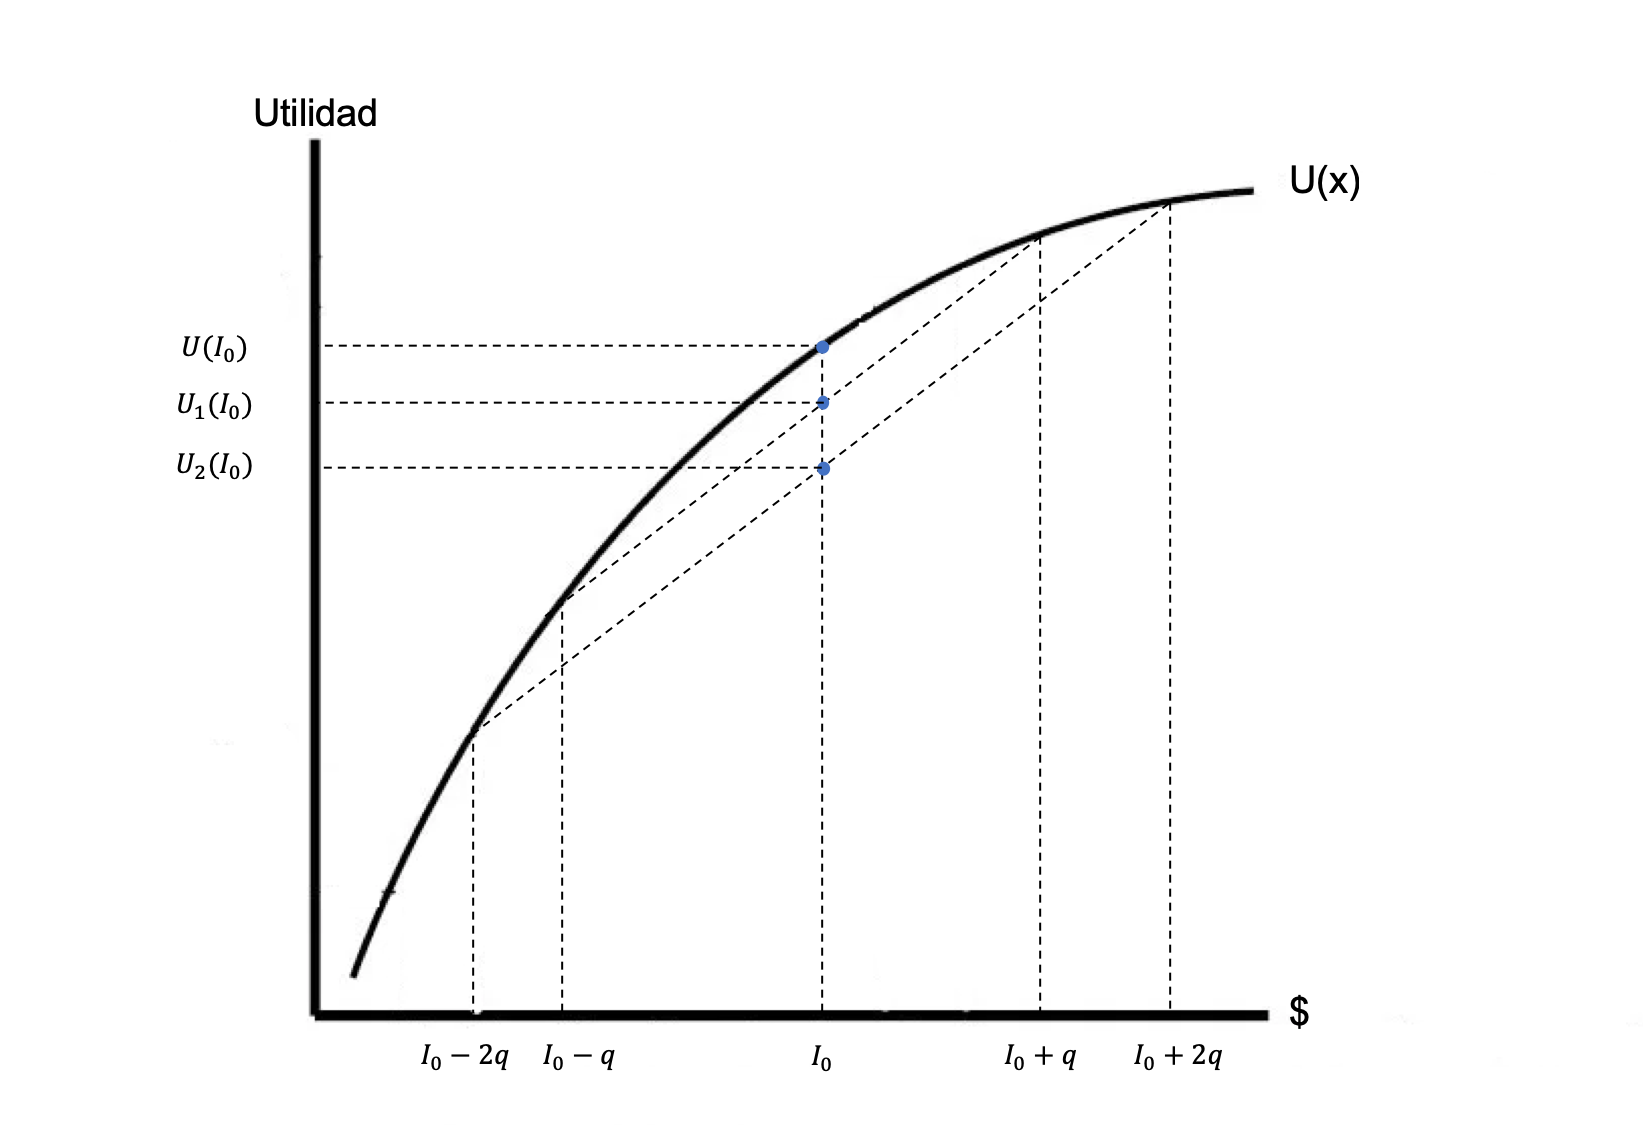
\includegraphics[scale = 0.43]{Imagenes/g1.png}
    \imagesource{Elaboración propia}
\end{figure}

Gráficamente podemos observar que:

$$
U(I_0) > U_{1}(I_0) > U_{2}(I_0)
$$

Con esto, podemos comprobar que un individuo averso al riesgo preferirá su riqueza inicial a jugar en una lotería justa y además preferirá una apuesta pequeña a una grande. También, se puede observar que cuando se tiene una riqueza menor, ganar el premio le genera mayor utilidad al individuo a comparación de la situación en donde la riqueza es mayor donde si se gana el premio la utilidad no aumenta de manera significativa. \\

Veamos un ejemplo numérico, supongamos que el indidividuo tiene una riqueza inicial $I_0 = \$100$ y se le propone apostar $\$80$ en un volado con una moneda honesta, por lo que la lotería quedaría definida de la siguiente manera:

\begin{table}[H]
\centering
\begin{tabular}{l|ll}
\cline{2-2}
    & x_1 = \$180 & con p_1 = \frac{1}{2} \\
L = &          &            \\
    & x_2 = \$20  & con p_2 = \frac{1}{2}  \\ \cline{2-2}
\end{tabular}
\end{table}

Observamos que, el valor esperado de la lotería $E[L] = \$100$ y tiene dos opciones:

\begin{itemize}
    \item No jugar y con probabilidad 1 tener $I_0 = \$100$ esto es $U(100)$
    \item Jugar la lotería y tener de utilidad esperada $UE[L] = p_1U(x_1) + p_2U(x_2)$ = $\frac{U(180)+U(20)}{2}$
\end{itemize} 

\newpage

Se tiene que, $U(100) > UE[L]$ esto debido a que al ser una función cóncava cualquier combinación lineal que se obtenga queda en el conjunto inferior dando una utilidad menor y por lo tanto prefiere no jugar. \\

Lo anterior se utilizará para comprobar que los individuos representativos que participan en estas loterías son aversos al riesgo y ver que tipo de loterías son (justas o injustas). Con ello se podrá entender de mejor manera si la decisión de participar o no en la lotería compensa el \textit{trade-off} entre el riesgo tomado y el valor esperado del premio potencial.

%VER SI ESTO LO DEJO O LO QUITO
%Por otro lado, supongamos a una persona que se enfrenta a una apuesta donde las probabilidades de ganar \$12 o perder \$10 son 50:50. El valor esperado es de \$1, la decisión de aceptar o no esta lotería involucra un \textit{trade-off}: aceptar la apuesta significa tomar riesgo, pero también implica un mayor valor esperado.

\newpage

\section{Aversión al riesgo y riqueza}

En la sección \textbf{1.1.3} se presenta la teoría de Arrow y Pratt donde se introduce una forma de medir cuantitativamente que tan averso al riesgo es un individuo. Con ello, surge la pregunta si la aversión al riesgo incrementa o disminuye dependiendo del nivel de riqueza con el que se cuenta. \\

Para poder dar una respuesta al cuestionamiento anterior, Arrow y Pratt presentan una familia de funciones para entender los cambios en la aversión al riesgo cuando la riqueza cambia. Respecto a  la medida de \textit{aversión al riesgo absoluto} existen 3 tipos de funciones:  CARA, DARA  y IARA las cuales presentan aversión al riesgo constante, decreciente y creciente respectivamente. \\

Algebráicamente lo anterior se obtiene de la derivada de la ecuación (1.6) para llegar a lo siguiente:

$$
r^{\prime}(W) = \left \{ \begin{matrix} <0  & \implies \mbox{DARA}
\\ = 0 & \implies \mbox{CARA} 
\\ >0 & \implies \mbox{IARA}

\end{matrix}\right.
$$ \\

Para entender de mejor forma esta familia de funciones, consideremos dos niveles de riqueza $W_1$ y $W_2$ con $W_1 > W_2$ y un posible pago monetario de $x$. Adicionalmente, supongamos $u(\cdot)$ una función de utilidad de tipo Bernoulli. \\

Un individuo con función de utilidad $u(\cdot)$ presenta aversión al riesgo absoluto decreciente (DARA) si:

\begin{equation}
    r(W_1 + x, u) < r(W_2 + x, u)
\end{equation}

Por otro lado, un individuo con función de utilidad $u(\cdot)$ presenta aversión al riesgo absoluto creciente (IARA) si:

\begin{equation}
    r(W_1 + x, u) > r(W_2 + x, u)
\end{equation}

Si tomamos ahora, una función de utilidad de la forma $u(W) = -e^{-\lambda W}$ con $\lambda > 0$ esta función de utilidad presenta aversión al riesgo absoluto constante (CARA) pues:

\begin{equation*}
    u^{\prime}(W)  & = \lambda e^{-\lambda W}, \: 
    u^{\prime \prime}(W) & = - \lambda^{2} e^{-\lambda W}
\end{equation*} 

\begin{equation*}
    \therefore r(W) = \lambda
\end{equation*}

Como se mencionó en la sección \textbf{1.1.3}, tratar de obtener estos coeficientes con los datos disponibles representa una dificultad dado que no se tiene una función de utilidad para cada individuo representativo de cada Estado y suponer una misma función de utilidad para todos no es lo ideal dado que no refleja la realidad. No se tomaría encuenta características ineherentes a cada Estado/Región que influyen en la percepción de la utilidad para cada individuo representativo. 

\newpage


\section{Elasticidades}
\noindent Una pregunta que se puede hacer en torno al ingreso y la cantidad demandada de un bien es cómo cambia el comportamiento de los individuos ante aumentos o disminuciones en el ingreso. ¿Consumirán más, menos o una cantidad igual de ese bien? \\

Para poder contestar la pregunta anterior defineremos a la elasticidad como \textit{una medida de sensibilidad que relaciona al precio o al ingreso con la cantidad demandada de un bien}. Utilizaremos este concepto debido a que, si bien es posible comparar las pendientes de diversas curvas de demanda, no siempre es lo óptimo puesto que estas pendientes dependen de las unidades en que medimos el precio y la cantidad y en ciertas ocasiones las unidades no están relacionadas. El concepto de elasticidad da la independecia de unidades. \\ 

Dentro de la teoría económica existen diferentes tipos de elasticidades, tales como: 

\begin{itemize}
    \item Elasticidad precio de la demanda
    \item Elasticidad precio de la oferta
    \item Elasticidad ingreso de la demanda
\end{itemize}

%per capita?
Para fines de esta tesis nos enfocaremos en la elasticidad ingreso para analizar los efectos y la sensibilidad existente entre la demanda de boletos del Sorteo Tec y el ingreso de los individuos representativos de cada Estado. Realizaremos un estudio similar a los que se describen en la sección \textbf{1.2 Revisión de literatura}. \\ 

Imaginemos dos situaciones, la primera donde la economía está en crecimiento y expansión, los individuos tienen ingresos más altos lo cual genera un aumento en la demanda de casi todos los bienes y servicios. La segunda, donde la economía se encuentra estancada o se empiezan a ver indicadores de que la economía empezará a decrecer, los individuos empiezan a tener menores ingresos lo cual genera una disminución en casi todos los bienes y servicios. \\

Para poder explicar que le pasará a la demanda de los bienes y servicios en ambas situaciones explicaremos a detalle la teoría asociada a las elasticidades. \\

La \textbf{elasticidad ingreso de la demanda}  es la medida de sensibilidad de la demanda de un bien ante un cambio en el ingreso, cuando los demás factores se mantienen constantes. Esta elasticidad se calcula de la siguiente forma:

$$
\varepsilon_I= \frac{ \Delta \% \: cantidad \: demandada}{\Delta \% \, ingreso}
$$

Dicha elasticidad ingreso puede ser positiva, negativa o cero:

\begin{itemize}
    \item $\varepsilon_I > 1$: bien \textit{superior} al ingreso
    \item $\varepsilon_I = 1$: bien con elasticidad ingreso unitaria
    \item $0 < \varepsilon_I < 1$: bien \textit{normal} al ingreso
    \item $\varepsilon_I = 0$: bien \textit{neutro} al ingreso
    \item $\varepsilon_I < 0$: bien \textit{inferior} al ingreso
\end{itemize}{}

Cuando un bien es superior al ingreso quiere decir que si el ingreso aumenta, la cantidad demandada aumenta en mayor proporción que el aumento en el ingreso. Cuando un bien es normal al ingreso quiere decir que si el ingreso aumenta, la cantidad demandada aumenta en menor proporción que el aumento en el ingreso y si un bien es inferior al ingreso, quiere decir que ante un aumento en el ingreso, la cantidad demandada de ese bien disminuye. \\

Así, buscaremos encontrar cuál es la elasticidad ingreso de los boletos del Sorteo Tec para determinar qué tipo de bien es. Esto se relacionará con la teoría de elección bajo incertidumbre y su relación con la teoría de utilidad esperada para poder determinar cómo es el comportamiento de los individuos representativos de cada Estado ante diferentes situaciones respecto al ingreso. \\



%====== Texto de la tesis de ejemplo
%\subsection{Cambios cerebrales y genéticos}

%\noindent Brizendine (2010) escribe que algunos científicos piensan que ciertas áreas del cerebro son como centros de actividad que mandan señales eléctricas a otras áreas del cerebro ocasionando un determinado comportamiento.\footnote{ Por ejemplo, en el hombre la corteza del cíngulo anterior pesa opciones, detecta conflicto y motiva decisiones. La unión temporoparietal busca soluciones rápidas y ante situaciones estresantes toma en cuenta la perspectiva de otros individuos. La corteza cingulada anterior rostral se encarga de procesar los errores sociales, como la aprobación o desaprobación de otros.}

%\begin{quote}
%    \small{Mientras que la distinción entre los cerebros de niños y niñas empieza biológicamente, estudios recientes muestran que es \textit{solo} el comienzo. La estructura cerebral no está escrita sobre piedra en el nacimiento ni al final de la infancia, como antes se creía, sino que continúa cambiando a lo largo de la vida. Más que ser inmutable, nuestros cerebros son mucho más plásticos y cambiables de lo que los científicos creían hace una década. El cerebro humano es también la máquina de aprendizaje más talentosa que conocemos. Así que nuestra cultura y el cómo nos enseñaron a comportarnos desempeñan un papel importante en el diseño y reestructura de nuestros cerebros (Brizendine 2010, 5-6).}
%\end{quote}

% Para citas muy largas es mejor el \begin{quote}

%\vspace{1em}
%\noindent \textbf{Hipótesis 3.} \hfill\begin{minipage}{\dimexpr\textwidth-3cm}
%\textit{La intensidad religiosa está relacionada negativamente con la innovación.}
%\end{minipage}
%\vspace{1em}

% Para plantear hipótesis

%\begin{table}[H]
%\centering
%\caption{Índices de modernidad y tradicionalismo}
%\label{PHEL}
%\begin{tabular}{|ccc|}
%\hline
% País & Índice de modernidad & Índice de tradicionalismo  \\ 
%\hline
%Alemania & 0.58 & 0.45 \\
%Austria & 0.55 & 0.49  \\
%Bélgica & 0.50 & 0.49  \\
%Canadá & 0.61 & 0.50 \\
%Dinamarca & 0.58 & 0.44 \\ 
%España & 0.47 & 0.62 \\
%Estados Unidos & 0.59 & 0.44  \\
%Finlandia & 0.62 & 0.38 \\
%Francia & 0.49 & 0.59 \\ 
%Holanda & 0.58 & 0.49 \\ 
%Irlanda & 0.54 & 0.59  \\
%Islandia & 0.63 & 0.54 \\
%Italia & 0.56 & 0.58  \\
%Japón & 0.42 & 0.48 \\
%Noruega & 0.53 & 0.44 \\
%Portugal & 0.50 & 0.71 \\ 
%Reino Unido & 0.56 & 0.54  \\
%Suecia & 0.62 & 0.51 \\
%Promedio & 0.58 & 0.51 \\
%\hline
%\end{tabular}

%\begin{tabular}{c}
%\footnotesize{Fuente: Bojilov y Phelps (2012).}
%\end{tabular}

%\end{table}

% Para diseñar tablas

%====== Acaba texto de tesis de ejemplo